\begin{fullwidth}
\chapter{\label{ch:super_syllables}
Experimental results}
\end{fullwidth}

\begin{chabstract}

In this chapter we report subjects behavioral performance ...

\end{chabstract}


\section{Behavioral performance}
%
The subjects had a behavioral performance above 97\% in both visual and auditory \emph{Pseudoword matching tasks}, except for \emph{Subject 05} that reported concentration span issues over all the acquisition.
Note that due to the experimental design structure, in which we only query few random samples, small score decrements can imply distraction over an important task segment.
\emph{Subjects 01 and 04} reported in the second auditory session that the volume was not high enough to be comfortable, although this did not reflect on their behavioral performance.
So we consider all subjects data apt to neuroimaging interpretation, with caution over \emph{Subject 05}. Behavioral performance details are provided in Table \ref{table:behavior}.


\begin{table}
\begin{tabular}{|>{\bfseries}l|rrr|}
\toprule
Subject &  Visual (\%) &  Auditory (\%) &  Overall (\%) \\
\midrule
01 &        97.22 &          97.22 &    97.22 \\
02 &       100.00 &          98.61 &    99.31 \\
03 &        97.92 &          97.22 &    97.57 \\
04 &        99.31 &          99.31 &    99.31 \\
05 &        92.36 &          88.89 &    90.62 \\
\bottomrule
\end{tabular}
\caption{\textbf{Behavioral performance on the \emph{Pseudowords matching task}:} Performance correspond to correctly identifying if the pseudowords were the same or different, with no answer considered as incorrect. Visual and Auditory headers refer to the sensory modality of the task, where overall is the mean performance of both modalities.}
\label{table:behavior}
\end{table}


\section{Sanity checks}\label{sec:sanity_checks}

\begin{figure*}[ht]
\scriptsize
\hspace{-4ex}
\begin{tabular}{ccc}
\textbf{\Large Subject 1} & \textbf{\Large Subject 2} & \textbf{\Large Subject 3}\\
{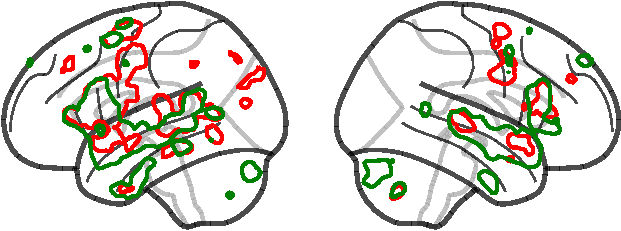
\includegraphics[width=.33\linewidth]{figures/part_II/langloc_01.pdf}}
\hspace{-1ex}
&{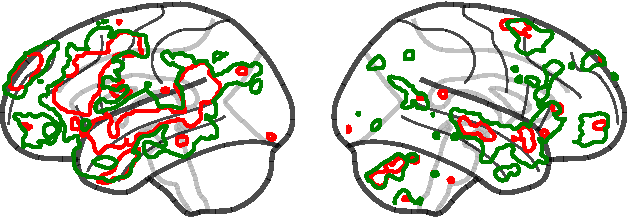
\includegraphics[width=.33\linewidth]{figures/part_II/langloc_03.pdf}}
\hspace{-1ex}
&{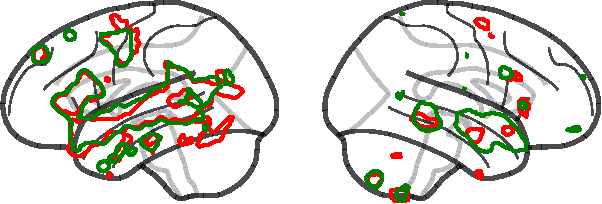
\includegraphics[width=.33\linewidth]{figures/part_II/langloc_04.pdf}}
\hspace{-1ex}\\
\rule{0pt}{6ex}
\textbf{\Large Subject 4} & \textbf{\Large Subject 5} & {}\\
{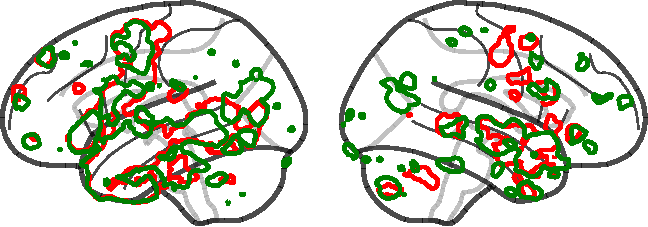
\includegraphics[width=.33\linewidth]{figures/part_II/langloc_05.pdf}}
\hspace{-1ex}
&{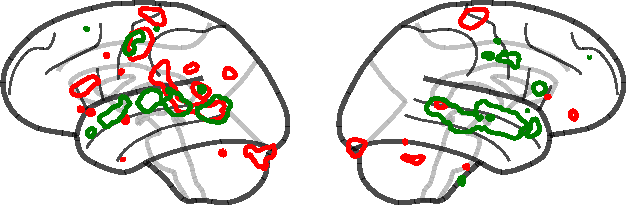
\includegraphics[width=.33\linewidth]{figures/part_II/langloc_06.pdf}}
\hspace{-1ex}
&{
\includegraphics[width=.2\linewidth]{figures/part_II/langloc_legend.pdf}}
\hspace{-1ex} \\
\end{tabular}
\vspace{0ex}
\caption{\textbf{Language localizers:} We show left and right hemispheric contours of the language localizer contrast of word sequences over control stimuli (consonant strings or scrambled recordings), thresholded at a p-value < 10e-3.
Statistical images are projected in the anatomical space of each subject.}
\label{fig:language_localizers}
\end{figure*}

\paragraph{Language localizer activations:}
The contours of the language localizers' contrasts, thresholded at p-value < 10e-3, for both auditory and visual modalities are presented in Figure \ref{fig:language_localizers} for all subjects.
We also show in Figure \ref{fig:language_localizers_radial} the coverage of Mahowald et al. parcels\citep{mahowald2016reliable} by the thresholded language localizers for all subjects.
We see observe an expected left lateralization of the detected language network with more than 40\% coverage of all the language parcels, which covers the fronto-temporal language system that has been well depicted in previous imaging studies\citep{mahowald2016reliable, fedorenko2010new, dehaene2010learning, binder1997human}.
There is variability between the modalities, that particularly disfavors activations of the visual one, in which the subjects can get distracted from perceiving and processing the stimuli more easily, than in the auditory case.
This could be expected from the intrinsic variability of different experimental designs in language localizers as demonstrated by Mahowald et al.\citep{mahowald2016reliable}.
\emph{Subjects 1 and 5} have a defficient coverage that will diminish our capacity to interpret syllabic representation effects along their cortex.
In particular \emph{Subject 5}, who reported concentration problems, have an extremely defficient coverage of the language network.

\begin{figure}[ht]
\scriptsize
\hspace{-4ex}
\begin{tabular}{ccc}
{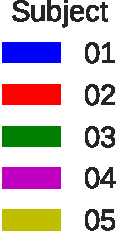
\includegraphics[width=0.1\linewidth]{figures/part_II/subjects_legend.pdf}}
\hspace{-1ex}
&{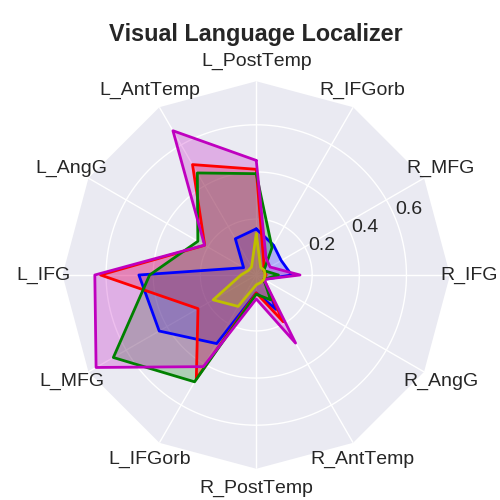
\includegraphics[width=0.45\linewidth]{figures/part_II/visual_langloc_radial.png}}
\hspace{-1ex}
&{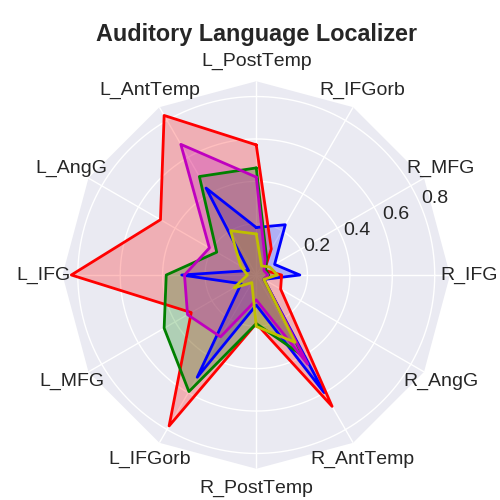
\includegraphics[width=0.45\linewidth]{figures/part_II/auditory_langloc_radial.png}}
\hspace{-1ex}\\
\end{tabular}
\caption{\textbf{Language localizer parcel coverage:}
We show the parcel coverage of each language localizer for the 6 language parcels derived by Mahowald et al. in both hemispheres.
Each subject is represented in a radial chart to emphasize the overall coverage of the language localizers of each subject.
Also the left and right hemisphere parcels have been arranged symmetrically in the radial charts.}
\label{fig:language_localizers_radial}
\end{figure}

\paragraph{Motor activations:}
We verified the integrity of the activation maps of the \emph{Pseudoword matching task} with statistical tests portraying the left and right hand button press contrast.
Z score maps of the left over right button press contrast, for all subjects, are shown in Figure \ref{fig:button_press}, confirming a good statistical separation of hand responses.

\begin{figure}[ht]
\scriptsize
\hspace{-4ex}
\begin{tabular}{cccccl}
\textbf{\Large Subject 1} & \textbf{\Large Subject 2} & \textbf{\Large Subject 3} & \textbf{\Large Subject 4} & \textbf{\Large Subject 5} & {}\\
{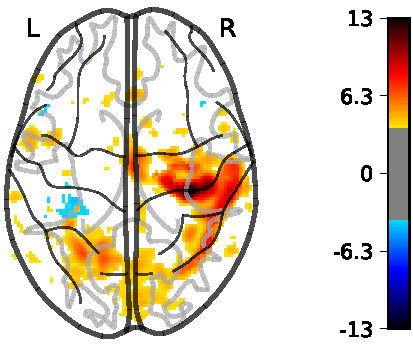
\includegraphics[width=.14\linewidth]{figures/part_II/press_vis_01.pdf}}
\hspace{1ex}
&{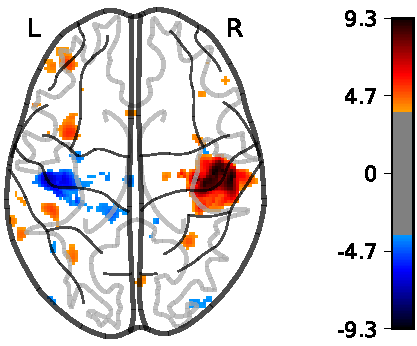
\includegraphics[width=.14\linewidth]{figures/part_II/press_vis_03.pdf}}
\hspace{1ex}
&{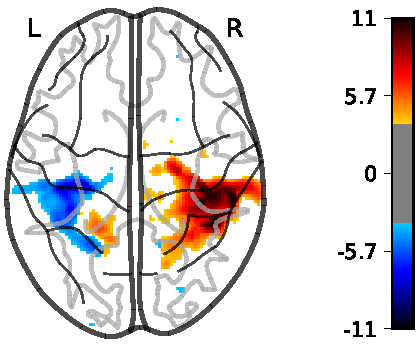
\includegraphics[width=.14\linewidth]{figures/part_II/press_vis_04.pdf}}
\hspace{1ex}
&{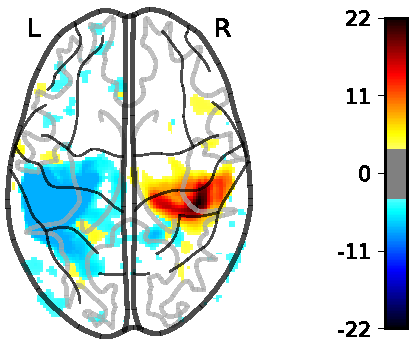
\includegraphics[width=.14\linewidth]{figures/part_II/press_vis_05.pdf}}
\hspace{1ex}
&{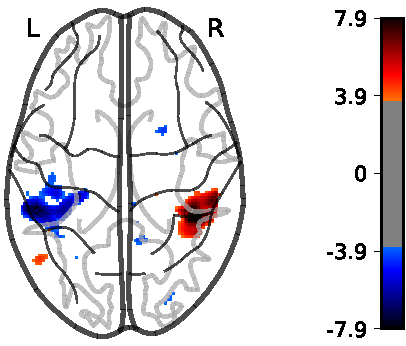
\includegraphics[width=.14\linewidth]{figures/part_II/press_vis_06.pdf}}
\hspace{1ex}
& {} \\
{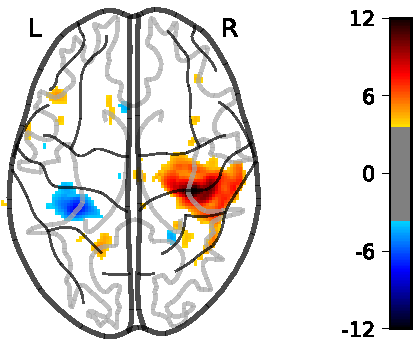
\includegraphics[width=.14\linewidth]{figures/part_II/press_aud_01.pdf}}
\hspace{1ex}
&{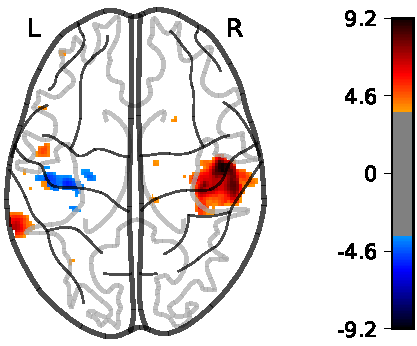
\includegraphics[width=.14\linewidth]{figures/part_II/press_aud_03.pdf}}
\hspace{1ex}
&{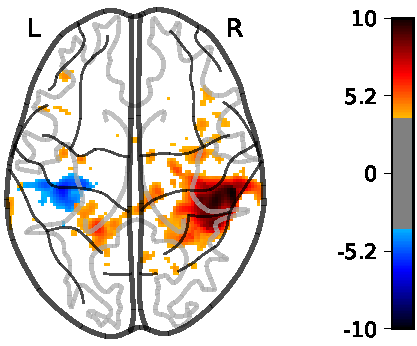
\includegraphics[width=.14\linewidth]{figures/part_II/press_aud_04.pdf}}
\hspace{1ex}
&{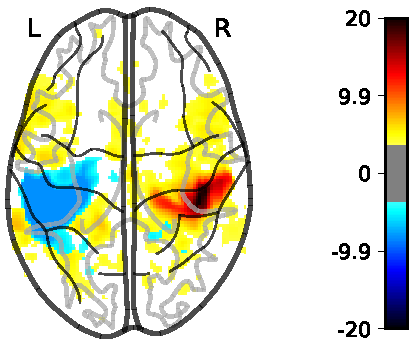
\includegraphics[width=.14\linewidth]{figures/part_II/press_aud_05.pdf}}
\hspace{1ex}
&{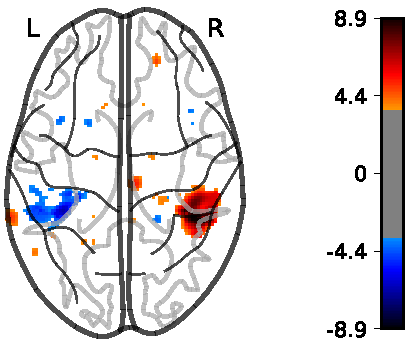
\includegraphics[width=.14\linewidth]{figures/part_II/press_aud_06.pdf}}
\hspace{1ex}
&{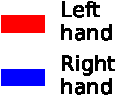
\includegraphics[width=.10\linewidth]{figures/part_II/press_legend.pdf}} \\
\end{tabular}
%\vspace{3ex}
\caption{\textbf{Button press effects:} We show the left button press over right button press contrast Z scores from the auditory modality, thresholded at p < 10e-4, for all subjects. Statistical images correspond to the anatomical space of each subject.}
\label{fig:button_press}
\end{figure}

We also verified that we can employ a Support Vector Classifier (SVC) to distinguish individual left and right button press activation maps derived from the \emph{Pseudoword matching task} General Linear Model (GLM).
As can be seen in Table \ref{table:clic}, we achieve high classification scores of right and left button press events for all subjects.
Moreover as would be expected, the classification generalize across sensory modalities.

\begin{table}
\begin{tabular}{|>{\bfseries}l|rrrrr|}
\toprule
(Train, Test) & (V, V) & (A, A) & (V, A) & (A, V) & (V-A, V-A) \\
Subject & (\%) &  (\%)   & (\%)  & (\%)  &   (\%)\\
\midrule
01      &   84.38*** &   93.50*** &   80.84*** &   76.94*** &           90.88*** \\
02      &   95.38*** &   92.50*** &   84.03*** &   93.03*** &           95.31*** \\
03      &   98.00*** &   99.00*** &   93.91*** &   98.75*** &          100.00*** \\
04      &   97.38*** &   99.50*** &   97.50*** &   98.72*** &          100.00*** \\
05      &   86.62*** &   77.62*** &   90.12*** &   74.28*** &           93.56*** \\
\bottomrule
\end{tabular}
\vspace{5ex}
\caption{\textbf{Classification of left and right button press maps of \emph{Pseudoword matching task}:} \emph{"V"} corresponds to the Visual modality and \emph{"A"} to the Auditory modality. \emph{"V-A"} corresponds to pooling together both datasets for training and testing.}
\label{table:clic}
\end{table}

\blankfootnote{\emph{chance: 50\% \\ * : p < 10e-2,\\ ** : p < 10e-3,\\ *** : p < 10e-4 \\ Bonferroni corrected for 25 similar tests performed}}

\paragraph{Visual activations:}
We verified the statistical effects of left and right syllable position in the Visual hOc1 region.
In the experimental design we asked the subjects to fixate a centered green dot before stimuli presentation.
So we expected, from well known retinotopic effects in the primary visual cortex \citep{tootell1998retinotopy}, to see an hemispheric partition of left and right syllable position effects, such that left syllable effects would be emphasized in the right hemisphere and right syllable effects in the left hemisphere.
This was the case, as can be seen in Figure \ref{fig:retinotopy}, where \emph{Subjects 1 and 4} have the clearest retinotopic activations.
Nonetheless we can also appreciate in the images that some subjects did not manage to completely follow the fixation instruction, since effects of both positions are present together in both hemispheres.


\begin{figure*}[ht]
\scriptsize
\vspace{2ex}
\hspace{-4ex}
\begin{tabular}{cccccl}
\textbf{\Large Subject 1} & \textbf{\Large Subject 2} & \textbf{\Large Subject 3} & \textbf{\Large Subject 4} & \textbf{\Large Subject 5} & {}\\
{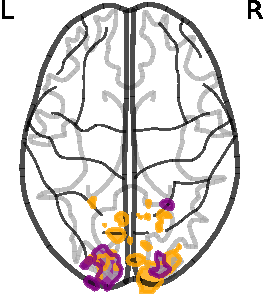
\includegraphics[width=.13\linewidth]{figures/part_II/retinotopy_01.pdf}}
\hspace{1ex}
&{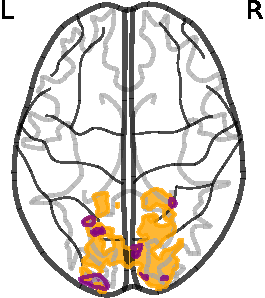
\includegraphics[width=.13\linewidth]{figures/part_II/retinotopy_03.pdf}}
\hspace{1ex}
&{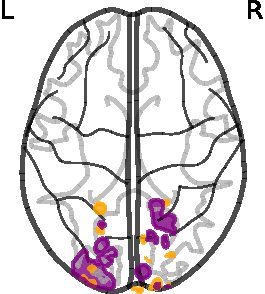
\includegraphics[width=.13\linewidth]{figures/part_II/retinotopy_04.pdf}}
\hspace{1ex}
&{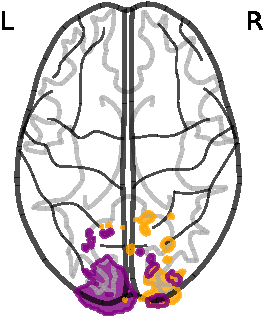
\includegraphics[width=.13\linewidth]{figures/part_II/retinotopy_05.pdf}}
\hspace{1ex}
&{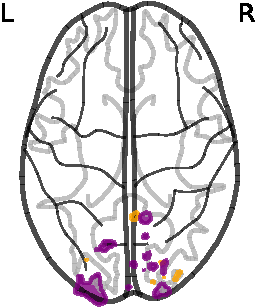
\includegraphics[width=.13\linewidth]{figures/part_II/retinotopy_06.pdf}}
\hspace{-1ex}
&{
\includegraphics[width=.12\linewidth]{figures/part_II/retinotopy_legend.pdf}}
\hspace{-1ex} \\
\end{tabular}
\vspace{3ex}
\caption{\textbf{Retinotopic effect:} We show first and second syllable position effects masked by the Visual hOc1 region, thresholded at a p-value < 0.005.
Statistical images correspond to the anatomical space of each subject.}
\label{fig:retinotopy}
\end{figure*}



\section{Visual representations}

Due to retinotopy and the large size of the text presented in the \emph{Pseudowords matching task}, we expected to be able to decode visual representations and demonstrate superposed representations trivially implied by retinotopy.

As can be seen in Table \ref{table:visual_word_pred}


\begin{figure}[ht]
\scriptsize
\vspace{2ex}
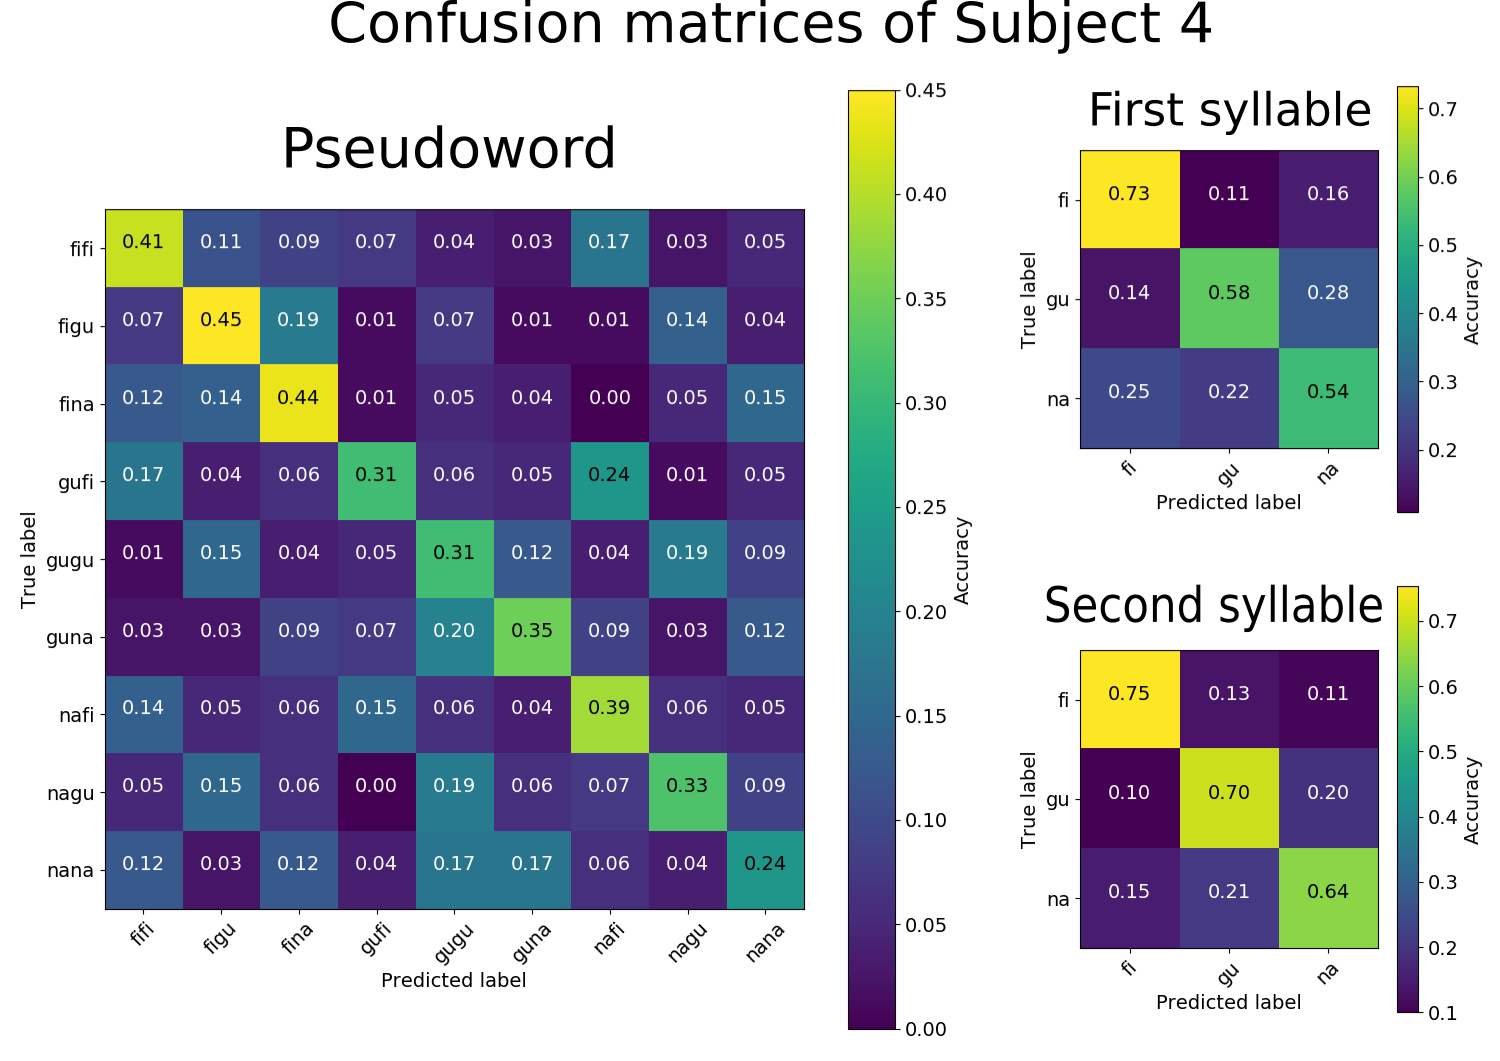
\includegraphics[width=1.\linewidth]{figures/part_II/confusion_subject_4.png}
\vspace{3ex}
\caption{\textbf{Confusion matrices of \emph{Subject 4}:}
We show }
\label{fig:visual_confusion}
\end{figure}


\begin{table*}
\begin{tabular}{lllllllllll}
\toprule
Condition &    fifi &    figu &    fina &    gufi &    gugu &    guna &    nafi &    nagu &    nana &    Mean \\
Subject &         &         &         &         &         &         &         &         &         &         \\
\midrule
01      &  0.30** &  0.23** &  0.29** &   0.19* &   0.19* &    0.15 &   0.16* &    0.12 &  0.20** &  0.20** \\
02      &    0.17 &   0.20* &   0.21* &    0.16 &    0.15 &    0.09 &  0.23** &   0.15* &    0.12 &  0.17** \\
03      &   0.25* &    0.19 &   0.21* &    0.14 &  0.17** &    0.12 &  0.19** &   0.14* &    0.11 &  0.17** \\
04      &  0.41** &  0.45** &  0.44** &  0.31** &  0.31** &  0.35** &  0.39** &  0.33** &  0.24** &  0.36** \\
05      &   0.20* &  0.23** &    0.16 &    0.14 &  0.20** &   0.16* &   0.15* &    0.14 &    0.11 &  0.17** \\
\bottomrule
\end{tabular}
\vspace{2ex}
\caption{\textbf{Classification of left and right button press maps of \emph{Pseudoword matching task}:} \emph{"V"} corresponds to the Visual modality and \emph{"A"} to the Auditory modality. \emph{"V-A"} corresponds to pooling together both datasets for training and testing.}
\label{table:visual_word_pred}
\end{table*}

\vspace{30ex}
\blankfootnote{\emph{chance: 50\% \\ * : p < 10e-2,\\ ** : p < 10e-3,\\ *** : p < 10e-4 \\}}


\begin{figure*}[ht]
\scriptsize
\vspace{2ex}
\hspace{-4ex}
\begin{tabular}{ccccc}
\textbf{\Large Subject 1} & \textbf{\Large Subject 2} & \textbf{\Large Subject 3} & \textbf{\Large Subject 4} & \textbf{\Large Subject 5}\\
{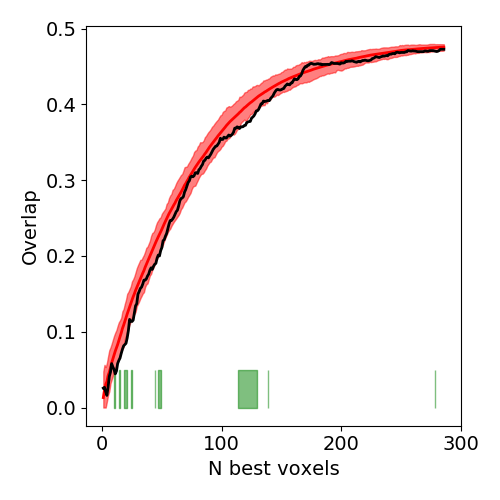
\includegraphics[width=.19\linewidth]{figures/part_II/locality_test_01.png}}
\hspace{0ex}
&{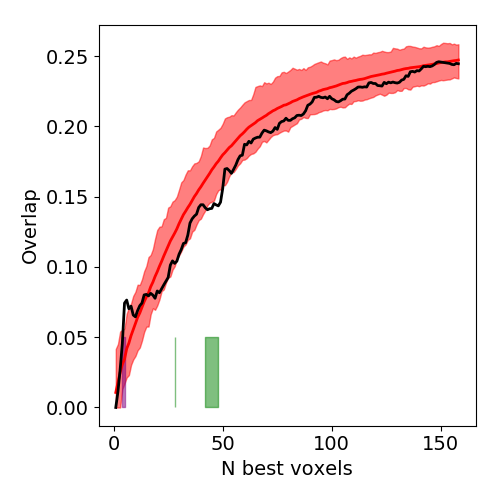
\includegraphics[width=.19\linewidth]{figures/part_II/locality_test_03.png}}
\hspace{0ex}
&{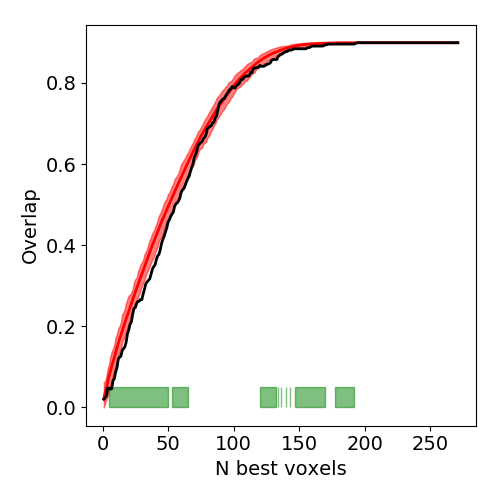
\includegraphics[width=.19\linewidth]{figures/part_II/locality_test_04.png}}
\hspace{0ex}
&{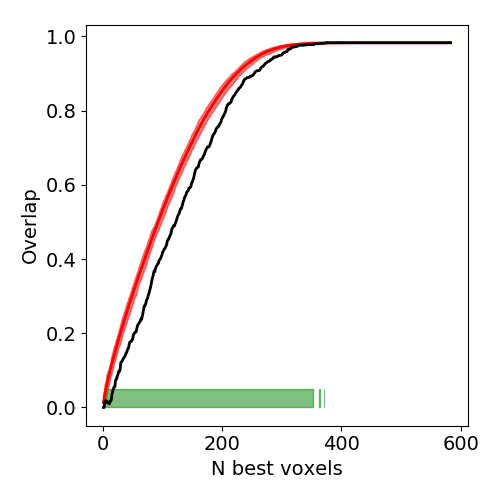
\includegraphics[width=.19\linewidth]{figures/part_II/locality_test_05.png}}
\hspace{0ex}
&{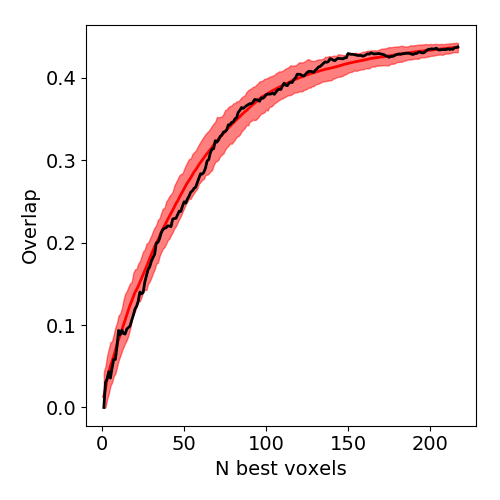
\includegraphics[width=.19\linewidth]{figures/part_II/locality_test_06.png}}
\hspace{-1ex} \\
\end{tabular}
\vspace{3ex}
\caption{\textbf{Partitioned spatial distribution of visual representations:} We show }
\label{fig:visual_locality}
\end{figure*}


\begin{table*}
\begin{tabular}{llllllllll}
\toprule
Test & Relatedness &          &        & No roles &         &        & Superposition &          &         \\
Overlap &        Diff & Position &   None &     Diff & Crossed &   None &          Diff & Position & Crossed \\
Subject &             &          &        &          &         &        &               &          &         \\
\midrule
01      &       0.018 &    0.115 &  0.097 &   -0.046 &   0.052 &  0.097 &       0.063** &    0.115 &   0.052 \\
02      &       0.000 &    0.000 &  0.000 &    0.000 &   0.000 &  0.000 &         0.023 &    0.110 &   0.088 \\
03      &       0.003 &    0.109 &  0.106 &    0.006 &   0.112 &  0.106 &        -0.003 &    0.109 &   0.112 \\
04      &     0.064** &    0.117 &  0.053 &   -0.018 &   0.035 &  0.053 &       0.082** &    0.117 &   0.035 \\
05      &       0.011 &    0.098 &  0.088 &    0.031 &   0.119 &  0.088 &        -0.020 &    0.098 &   0.119 \\
\bottomrule
\end{tabular}
\vspace{10ex}
\caption{\textbf{Classification of left and right button press maps of \emph{Pseudoword matching task}:} \emph{"V"} corresponds to the Visual modality and \emph{"A"} to the Auditory modality. \emph{"V-A"} corresponds to pooling together both datasets for training and testing.}
\label{table:superposition tests}
\end{table*}

\vspace{40ex}
\blankfootnote{\emph{chance: 50\% \\ * : p < 10e-2,\\ ** : p < 10e-3,\\ *** : p < 10e-4 \\ Bonferroni corrected for 25 similar tests performed}}



\section{Auditory representations}






% \section{Language representations}


% \paragraph{\emph{Pseudoword matching task} effects:}
% Neural activations related to differences between the nine bi-syllabic conditions are spread across the cortex for all subjects, as reveals the simple check of the contour of an F test, thresholded at p-value < 0.0001, of any difference between conditions, shown in Figure \ref{fig:any-effects}.
% Nonetheless, to pursue the objective of this work, we needed to separate regions encoding the stimuli as a whole (holistic representation) from regions encoding stimuli parts (distributed representation) that might further follow the superposition principle (superposed representation).
% From an statistical point of view, this means that we wanted to discriminate regions on which there are only effects of the first and second syllable position from regions on which there is an interaction effect that would suggest additional encoding terms contradicting the superposition principle.
% In Figure \ref{fig:syllable_effects} we pool together the filled contours of the statistical effects, thresholded at p-value < 0.0001, of any syllable position and their interaction from both auditory and visual modalities.
% From the high level perspective of Figure \ref{fig:syllable_effects}, we can observe that all effects spread around the whole brain and then occupy similar functional regions in all subjects, although position effects seem to occupy a higher portion of the cortex.

% \begin{figure}[ht]
% \scriptsize
% \vspace{5ex}
% \hspace{-4ex}
% \begin{tabular}{ccccc}
% \textbf{\Large Subject 1} & \textbf{\Large Subject 2} & \textbf{\Large Subject 3} & \textbf{\Large Subject 4} & \textbf{\Large Subject 5}\\
% {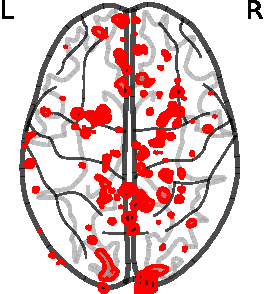
\includegraphics[width=.165\linewidth]{figures/part_II/any-effects_01.pdf}}
% \hspace{1ex}
% &{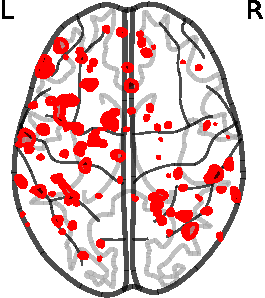
\includegraphics[width=.165\linewidth]{figures/part_II/any-effects_03.pdf}}
% \hspace{1ex}
% &{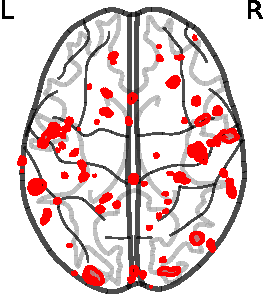
\includegraphics[width=.165\linewidth]{figures/part_II/any-effects_04.pdf}}
% \hspace{1ex}
% &{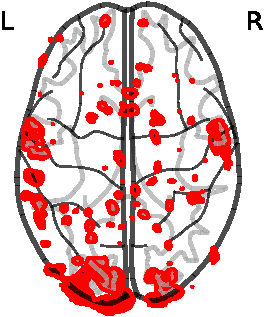
\includegraphics[width=.165\linewidth]{figures/part_II/any-effects_05.pdf}}
% \hspace{1ex}
% &{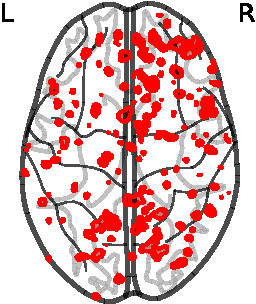
\includegraphics[width=.165\linewidth]{figures/part_II/any-effects_06.pdf}}
% \hspace{1ex}\\
% \end{tabular}
% \vspace{3ex}
% \caption{\textbf{Any stimuli difference:} We show the contour of the statistical F test reflecting any difference between the bi-syllabic conditions, thresholded at a p-value < 0.0001. Statistical images correspond to the anatomical space of each subject.}
% \label{fig:any-effects}
% \end{figure}


% \begin{figure*}[ht]
% \scriptsize
% \hspace{-4ex}
% \begin{tabular}{ccc}
% \textbf{\Large Subject 1} & \textbf{\Large Subject 2} & \textbf{\Large Subject 3}\\
% {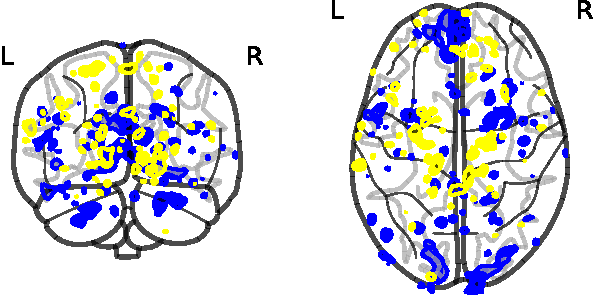
\includegraphics[width=.33\linewidth]{figures/part_II/all-effects_01.pdf}}
% \hspace{-1ex}
% &{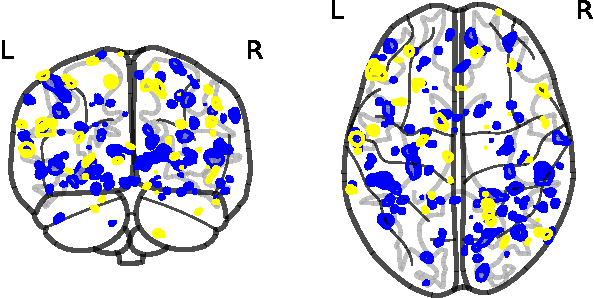
\includegraphics[width=.33\linewidth]{figures/part_II/all-effects_03.pdf}}
% \hspace{-1ex}
% &{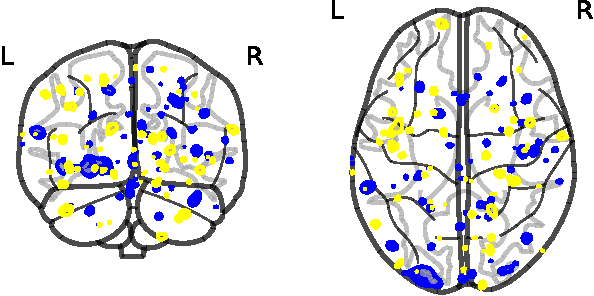
\includegraphics[width=.33\linewidth]{figures/part_II/all-effects_04.pdf}}
% \hspace{-1ex}\\
% \rule{0pt}{6ex}
% \textbf{\Large Subject 4} & \textbf{\Large Subject 5} & {}\\
% {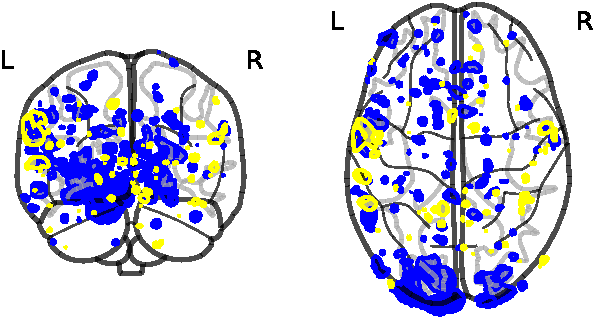
\includegraphics[width=.33\linewidth]{figures/part_II/all-effects_05.pdf}}
% \hspace{-1ex}
% &{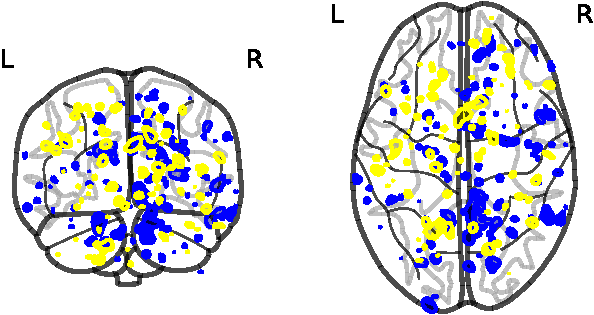
\includegraphics[width=.33\linewidth]{figures/part_II/all-effects_06.pdf}}
% \hspace{-1ex}
% &{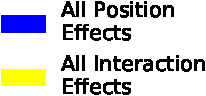
\includegraphics[width=.2\linewidth]{figures/part_II/all-effects_legend.pdf}}
% \hspace{-1ex} \\
% \end{tabular}
% \vspace{3ex}
% \caption{\textbf{Pseudoword matching task effects:} We show blobs corresponding to the statistical test of main effects (effect of first and second position) and interaction (sign of holistic representation) for the \emph{Pseudoword matching task}, thresholded at a p-value < 0.0001.
% We consider blobs from both auditory and visual modalities of the task together, to portray the extent of the possible effects. Statistical images correspond to in the anatomical space of each subject.}
% \label{fig:syllable_effects}
% \end{figure*}


% \paragraph{Searchlight networks derived:}
% Since we designed our stimuli to be interpreted from the point of view of morphological processing (language processing), we employed the statistical effect maps from both modalities to determine a sub-network of the identified language network in each subject that would be used for further classification with the searchlight procedure presented in the methods section \ref{sec:searchlight_classification}.
% We show in in Figure \ref{fig:searchlight_regions} the obtained searchlight networks for each subject, while emphasizing that both holistic and superposed representation candidate regions are captured inside the identified language networks.
% Notice that both candidates are spread on the whole fronto-temporal language system and that \emph{Subjects 2 and 4} have broad searchlight networks corresponding to their broader language network activations, as depicted in Figure \ref{fig:language_localizers}.


% \begin{figure}[ht]
% \scriptsize
% \hspace{-4ex}
% \begin{tabular}{cc}
% \textbf{\Large Subject 1} & \textbf{\Large Subject 2}\\
% {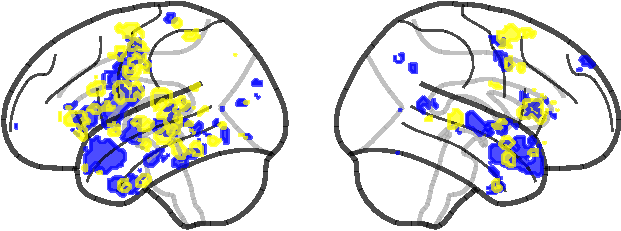
\includegraphics[width=.5\linewidth]{figures/part_II/searchlight-regions_01.pdf}}
% \hspace{-1ex}
% &{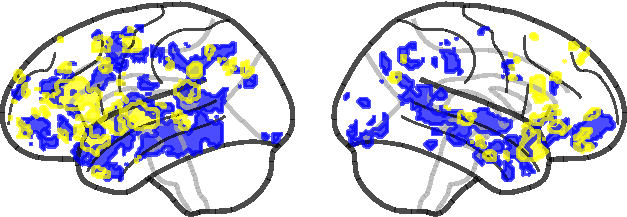
\includegraphics[width=.5\linewidth]{figures/part_II/searchlight-regions_03.pdf}}
% \hspace{-1ex}\\
% \rule{0pt}{6ex}
% \textbf{\Large Subject 3} & \textbf{\Large Subject 4}\\
% {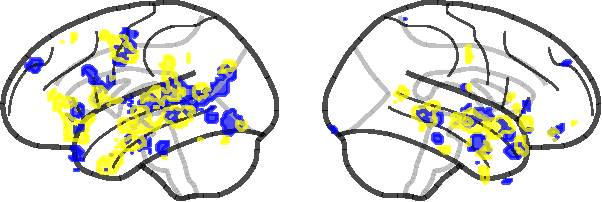
\includegraphics[width=.5\linewidth]{figures/part_II/searchlight-regions_04.pdf}}
% \hspace{-1ex}
% &{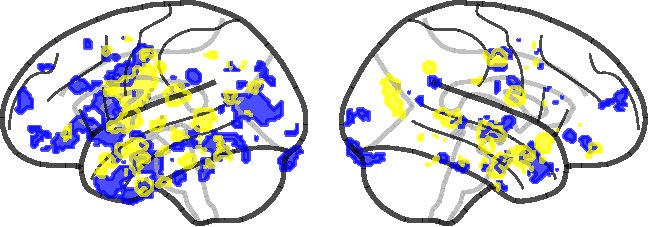
\includegraphics[width=.5\linewidth]{figures/part_II/searchlight-regions_05.pdf}}
% \hspace{-1ex}\\
% \rule{0pt}{6ex}
% \textbf{\Large Subject 5} & {}\\
% {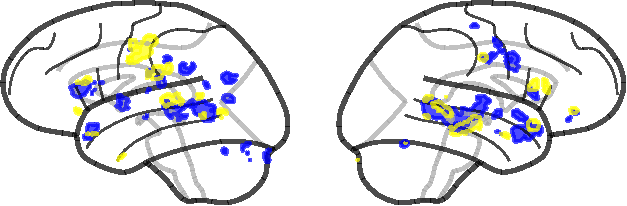
\includegraphics[width=.5\linewidth]{figures/part_II/searchlight-regions_06.pdf}}
% \hspace{-1ex}
% &{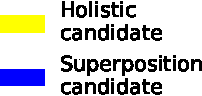
\includegraphics[width=.3\linewidth]{figures/part_II/searchlight-regions_legend.pdf}}
% \hspace{-1ex} \\
% \end{tabular}
% \vspace{3ex}
% \caption{\textbf{Searchlight networks:} We show the derived searchlight network for each subject. We separate for illustrative purposes the portion of the network derived from interaction effects (Holistic candidate) and from exclusive main effects (Superposition candidate). Images correspond to the anatomical space of each subject.}
% \label{fig:searchlight_regions}
% \end{figure}
